\documentclass[tikz,border=10pt]{standalone}
\begin{document}
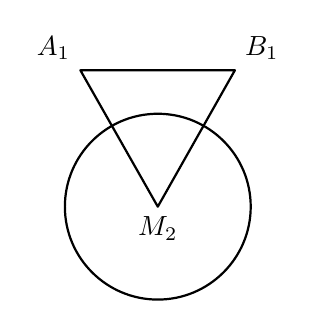
\begin{tikzpicture}[line width=0.8pt, line join=round]
% Coordinates: x = px/100, y = (221.2 - py)/100, so y=0 sits at M_2
\coordinate (A1) at (0.794,1.732);
\coordinate (B1) at (2.756,1.732);
\coordinate (M2) at (1.777,0);

% Full circle centred at M_2, radius 1.18 (units of 100 px)
\draw (M2) circle (1.18);

% Solid triangle sides A_1B_1, B_1M_2, M_2A_1
\draw (A1) -- (B1) -- (M2) -- cycle;

% Labels
\node[above left] at (A1) {$A_1$};
\node[above right] at (B1) {$B_1$};
\node[below] at (M2) {$M_2$};
\end{tikzpicture}
\end{document}